\section{Methods}
%describe the methods, the data, the assumptions, the scenarios, a brief few 
%sentences on Temoa itself.
Our current model leverages a robust dataset that populates multiple analytic 
models, trained neural networks, and  the Temoa framework (Tools for Energy 
Model Optimization and Analysis). Temoa is an open-source framework for 
simulating and optimizing energy systems. With our UIUC microgrid model in 
Temoa (Figure 1), we are able to determine the optimal energy generation mix 
for the UIUC microgrid for various objective functions (minimize carbon, 
minimize cost, etc.) while meeting system constraints (zero carbon by 2050, 
practical deployment speeds, realistic improvements in storage technology 
capabilities, etc.). The UIUC microgrid model includes transportation as well 
as campus steam, electric, and chilled water demand and provides cross-decadal 
deployment solutions which optimize the scenario objective function (Figure 2).

This model is underpinned by multiple advanced techniques. For example, a 
predictive model of net electricity demand on campus has been created with an 
echo state network machine learning approach to generate representative 
synthetic predictions of net grid load (Figure 3). This predictive model 
incorporates weather information to account for solar and wind power generation 
as well as heating and air-conditioning demands. Such predictive models are 
trained using multi-year historic campus electricity generation and consumption 
data. A similar approach will be used in the proposed simulations of the state 
as a whole.

\subsection{Generated Waste Data}
***description of waste calculator notebook for nuclear/wind/solar***

Coal power plants primarily produce solid wastes in the form of ash and slurries from the scrubbers.  Coal ash is produced from coal burning in approximately a 6:1 burned coal:coal ash ratio.  While the solid wastes are comprised of multiple elements, the waste is generally half coal ash, and half anhydrite ($CaSO_4$) - a product of chemical reactions in the scrubbers \cite{brown_solid_1996}.

\begin{figure}[h!]
\centering
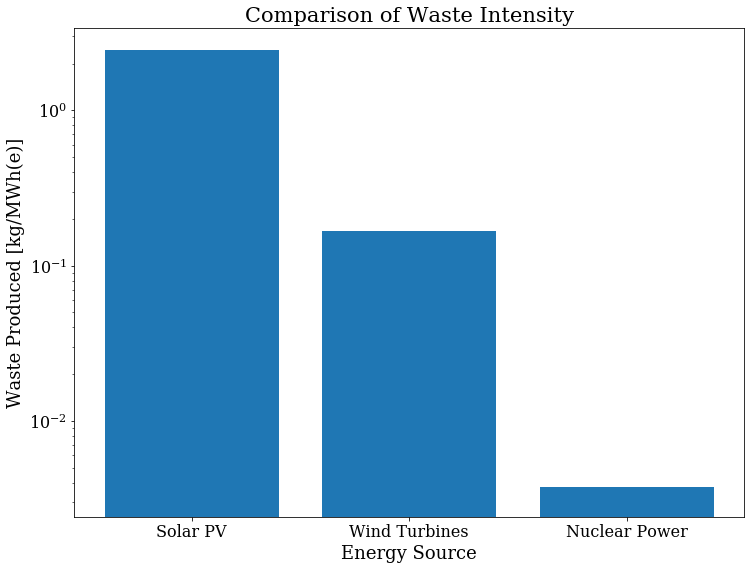
\includegraphics[width = 10cm]{img/mass-waste-intensity.png}
\caption{Solid Waste in $\frac{kg}{MWh}$ by Energy Source}
\label{fig:mass-waste}
\end{figure}



